
\begin{figure}[H]
\begin{center}
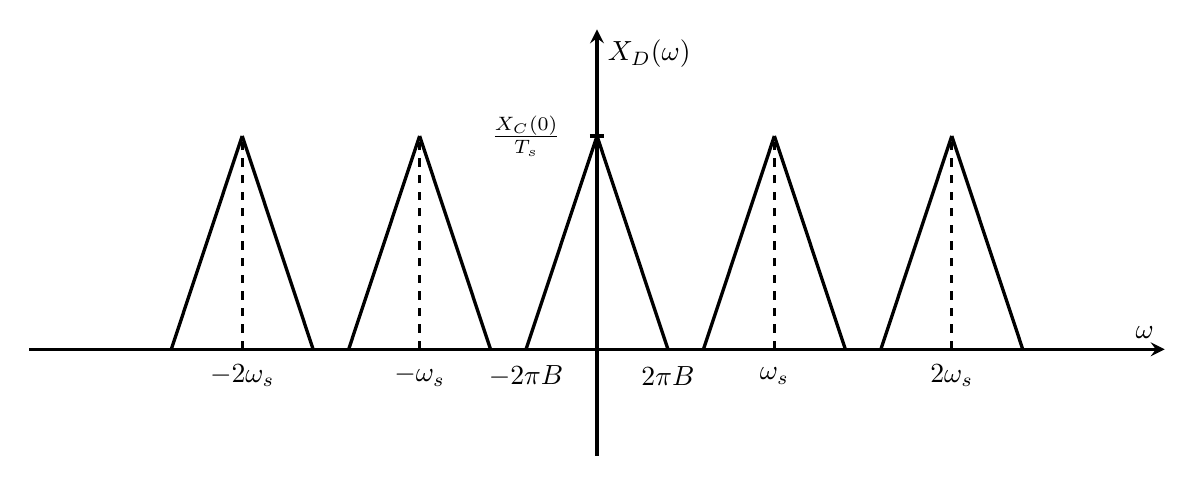
\begin{tikzpicture} 
\tikzset{every pin edge/.style={scale=0.00001}}
\begin{axis}[very thick,
                     samples = 100,
                     ytick={-2,2},
                     xlabel = {$\omega$},
                     ylabel = {$X_D(\omega)$},
                     xmin = -8,
                     xmax = 8,
                     ymin = -0.5,
                     ymax = 1.5,
                     width=16cm,
                     height=7cm,
                     axis x line = middle,
                     axis y line = middle,
                     ticks = none]
            \edef\mya{-5}
            \foreach \x in {1,2,...,5}
            {   
                \addplot[mark=none] coordinates {(\mya-1,0) (\mya,1)};
                \addplot[mark=none] coordinates {(\mya,1) (\mya+1,0)};
                \pgfmathparse{\mya+2.5}
                \xdef\mya{\pgfmathresult}
            }   
            \addplot[mark=none] coordinates {(-0.1,1) (0.1,1)};
            \node at (axis cs:-1,1){$\frac{X_C(0)}{T_s}$};
            \node at (axis cs:1,-0.125){$2\pi B$};
            \node at (axis cs:-1,-0.125){$-2\pi B$};
            \node at (axis cs:2.5,-0.125){$\omega_s$};
            \node at (axis cs:5,-0.125){$2\omega_s$};
            \node at (axis cs:-2.5,-0.125){$-\omega_s$};
            \node at (axis cs:-5,-0.125){$-2\omega_s$};
            
            \addplot[dashed] coordinates {(-5,0) (-5,1)};
            \addplot[dashed] coordinates {(-2.5,0) (-2.5,1)};
            \addplot[dashed] coordinates {(2.5,0) (2.5,1)};
            \addplot[dashed] coordinates {(5,0) (5,1)};
        \end{axis}
\end{tikzpicture}
\end{center}
\caption{Espectro de magnitude de $X_D(\omega)$. Sendo $B$ dado em Hz. Fonte: própria.}
\label{graph:2} 
\end{figure}